\begin{frame}[fragile]{Using UHD from Python (5/7)}

\footnotesize

\begin{itemize}
    \item \textbf{\textcolor{DarkBlue}{Step 5: Running the Python Receiver Application}}
\end{itemize}

\hspace{2.8em}
\parbox{0.88\linewidth}{
\footnotesize
Execute the Python application by specifying the receive frequency,
sample rate, capture duration, output filename, and receiver gain.
}

\vspace{0.2cm}

\scriptsize
\begin{Verbatim}[xleftmargin=3.8em,breaklines,breaksymbolleft={},breaksymbolright={}]
python3 basic_rx_B210.py -f 100e6 -r 1e6 -d 5 -o rx_b210.npy -g 70
\end{Verbatim}

\vspace{0.2cm}
\begin{itemize}
    \begin{itemize}
        \scriptsize
        \item The captured IQ samples are stored in the specified
        \texttt{.npy} file.
        \item The terminal displays the total number of samples received,
        confirming successful data capture.
    \end{itemize}
\end{itemize}
\vspace{0.3cm}

\begin{center}
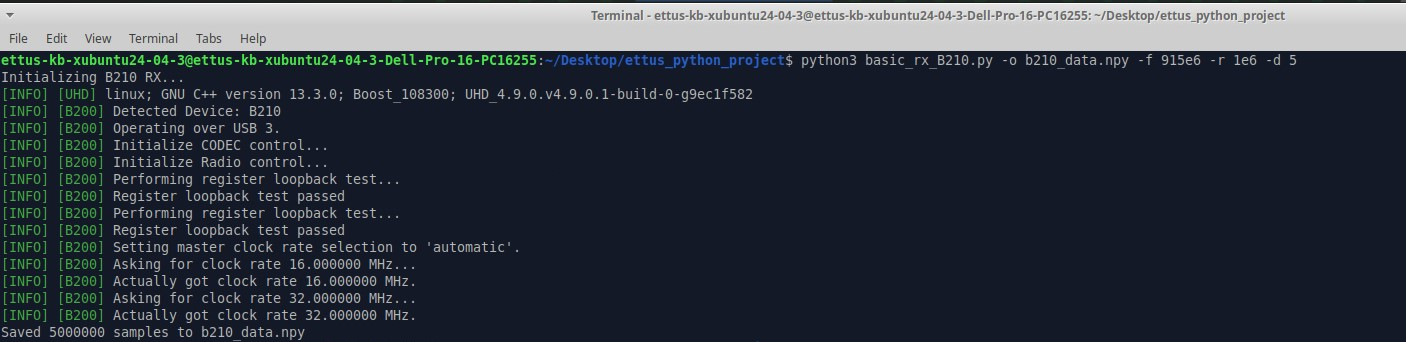
\includegraphics[width=0.90\linewidth,height=0.42\textheight,keepaspectratio]
{latex/jpg_png/image_python_api_B210_code_usage.jpg}
\end{center}

\end{frame}